
\documentclass[a4paper,UKenglish,cleveref, autoref]{lipics-v2019}
%This is a template for producing LIPIcs articles.
%See lipics-manual.pdf for further information.
%for A4 paper format use option "a4paper", for US-letter use option "letterpaper"
%for british hyphenation rules use option "UKenglish", for american hyphenation rules use option "USenglish"
%for section-numbered lemmas etc., use "numberwithinsect"
%for enabling cleveref support, use "cleveref"
%for enabling cleveref support, use "autoref"

\usepackage{wrapfig}
\usepackage[algo2e,vlined]{algorithm2e}

%\graphicspath{{./graphics/}}%helpful if your graphic files are in another directory

\bibliographystyle{plainurl}% the mandatory bibstyle

\title{A* with Perfect Potentials} %TODO Please add

% \titlerunning{Dummy short title}%optional, please use if title is longer than one line

\author{Ben Strasser}{Germany}{academia@ben-strasser.net}{TODO}{}%TODO mandatory, please use full name; only 1 author per \author macro; first two parameters are mandatory, other parameters can be empty. Please provide at least the name of the affiliation and the country. The full address is optional

\author{Tim Zeitz}{Institute of Theoretical Informatics, Algorithmics I, Karlsruhe Institute of Technology, Germany}{tim.zeitz@kit.edu}{}{}

\authorrunning{B. Strasser and T. Zeitz}%TODO mandatory. First: Use abbreviated first/middle names. Second (only in severe cases): Use first author plus 'et al.'

\Copyright{Ben Strasser and Tim Zeitz}%TODO mandatory, please use full first names. LIPIcs license is "CC-BY";  http://creativecommons.org/licenses/by/3.0/

\ccsdesc[500]{Theory of computation~Shortest paths}
% \ccsdesc[500]{General and reference}%TODO mandatory: Please choose ACM 2012 classifications from https://dl.acm.org/ccs/ccs_flat.cfm

\keywords{shortest path, road graphs, goal-directed search, contraction hierarchy}%TODO mandatory; please add comma-separated list of keywords

% \category{}%optional, e.g. invited paper

% \relatedversion{}%optional, e.g. full version hosted on arXiv, HAL, or other respository/website
%\relatedversion{A full version of the paper is available at \url{...}.}

% \supplement{}%optional, e.g. related research data, source code, ... hosted on a repository like zenodo, figshare, GitHub, ...

%\funding{(Optional) general funding statement \dots}%optional, to capture a funding statement, which applies to all authors. Please enter author specific funding statements as fifth argument of the \author macro.

% \acknowledgements{I want to thank \dots}%optional

%\nolinenumbers %uncomment to disable line numbering

%\hideLIPIcs  %uncomment to remove references to LIPIcs series (logo, DOI, ...), e.g. when preparing a pre-final version to be uploaded to arXiv or another public repository

%Editor-only macros:: begin (do not touch as author)%%%%%%%%%%%%%%%%%%%%%%%%%%%%%%%%%%
% \EventEditors{John Q. Open and Joan R. Access}
% \EventNoEds{2}
% \EventLongTitle{42nd Conference on Very Important Topics (CVIT 2016)}
% \EventShortTitle{CVIT 2016}
% \EventAcronym{CVIT}
% \EventYear{2016}
% \EventDate{December 24--27, 2016}
% \EventLocation{Little Whinging, United Kingdom}
% \EventLogo{}
% \SeriesVolume{42}
% \ArticleNo{23}
%%%%%%%%%%%%%%%%%%%%%%%%%%%%%%%%%%%%%%%%%%%%%%%%%%%%%%

\hideLIPIcs
\nolinenumbers

\begin{document}

\maketitle

\begin{abstract}
Efficiently computing flexible and optimal routes in continental-sized road networks is a tough challenge.
While Dijkstra's algorithm can be used to solve these problems, it is too slow for many practical applications.
A* is the classical approach to accelerate Dijkstra's algorithm and is used in many fields such as Experimental Algorithms, Robotics, or Artificial Intelligence.
However, A*'s performance depends on the availability of a good potential, also called heuristic, function.
Computing a good potential is a challenge of its own.
To avoid the need for a potential, many hierachical speedup techniques have been developped.
They achieve speed and optimality but sacrifize flexibility.
In this paper, we use hierarchical techniques to compute potential functions.
With this approach, we combine some of the hierarchical speed with the flexibility offered by A* - the best of both worlds - while retaining optimality.
\end{abstract}

\section{Introduction}
\label{sec:intro}
Route planning in street networks of continental scale is a well-researched topic with many applications~\cite{bdgmpsww-rptn-16}.
It is usually formalized as a variant of the classical shortest path problem in weighted graphs.
Efficiently computing flexible and optimal routes is a thought challenge.
Optimal means that the computed path always has minimum weight.
Efficiently means that the path computation is fast.
Being able to change the edge weights between path computations is flexibility.

Dijkstra's algorithm \cite{?} achieves flexiblity and optimality but unfortunately rrequires several seconds to compute paths across continental road networks, which is too slow for many applications.
A classic speedup approach is the well-known A* algorithm \cite{hnr-afbhd-68}.
While flexible, A*'s performance crucially depends on the quality of the potential, also called heuristic, function.
Finding such a function that can be computed efficiently is difficult.
A lot of research of the last decade has therefore focused on mostly hierarchical approaches \cite{CH,CCH,CRP,HIGHWAYHIERACHIES,MLD} which do not require such a function.
A popular hierachical algorithm is Contraction Hierarchy (CH) \cite{geisberger}.
There is a lot of work that extends CH to handle more complex settings.
For example, in \cite{sabine, kobitzsch} multi-criteria optimization is studied.
In \cite{CCH}, CH is modified to support Live-Traffic.
Historic traffic patterns are combined with CH in \cite{TD-CCH-preprint, TDCH, TDCRP}.
Specialized variants for electric vehicle routing are developped in \cite{moritz baum, charge}.
While these works show that it is possible to extend hierarchical approaches, they also show that it is non-trivial.
Further, in every setting the flexibility available at query time is fairly limited and usually encompasses only one very specific setting.

While undoubtedly fast, hierarchical approaches tend to sacrifice flexibility to obtain speed.
In this paper, we explore CH-Potentials, a novel combination of A* and the hierachical techniques CH and CCH.
We are not the first to combine hierarchical approaches and A* \cite{core-alt, real, charge, bdsssw-chgds-08}.
However, past work mostly uses A* to accelerate hierarchical approaches and sacrifzies A*'s felxibility in the process.
Our primary algorithm design objective is to retain A*'s flexibility.

Our algorithm is built upon ideas from Phast \cite{?}, a CH-extension.
The novel idea is to compute optimal A* potentials lazily.
The hierarchical approach is applied to the lower bound graph with respect to the edge costs.
As the hierarchical approaches are optimal, the resulting A* potential is the tightest possible.
With this approach, we combine some of the hierarchical speed with the flexibility offered by A* - the best of both worlds - while retaining optimality.
Figure~\ref{img:search-space} depicts an example  A* search with CH-Potentials.

\begin{figure}
TODO

\caption{Example search space when TODO: what parametrization?}
\label{img:search-space}
\end{figure}

Our technique can be applied to a CH and a CCH.
We describe our work mostly in CH terms.
Fortunately, all results are also directly applicable to CCH.
We describe the trade-off between the two variants in Section \ref{TODO}.

\section{Applications - Or why do we care about Flexibility?}

Modelling navigation as shortest path problem in graphs with scalar weights is a good but not perfect formalization.
Several important effects are ignored.
In this section, we list a few to motivate why flexibility is important.

The travel time across an edge is in general not constant over time.
Live-traffic and historic traffic patterns are examples of how the travel time can change.
Another example are road blockages.
These are usually modelled by setting travel times to infinity.
Some blockage types, such as accidents, are similar to live traffic.
Other blockages such as reversible one-ways, time-dependent turn-restrictions, or seasonal closures are more similar to historic traffic patterns.

Flexibility is also necessary to account for driver preferences.
For example, common options in navigation devices include avoiding highways or tunnels.
These requirements are usally modelled by modifying the edge weights and are highly depend on the driver.
Sometimes they even depend on his current mood and might change while driving.

Trucks are another class of vehicles with diverse and specific needs.
For example, trucks are not allowed in some areas depending on the time of the day.
Some truck carry hazardous materials and are therefore not allowed in some areas because of environmental protection laws.
Once the truck has delivered his goods, he may again pass the area.

\section{Problem Setting}

As detailed in the previous section, the reasons why flexibility is a necessary property of a routing engine are sheer endless.
However, a formal problem specification that encompasses all these options is complex and well beyond the scope of this paper.
For an example of such a formulation, we refer to \cite{sea2020paper} which covers a truck-specific application.
The algorithm presented in \cite{sea2020paper} uses a preliminary version of CH-Potentials.
For simplicity, we limit our exposition to the classical shortest path formulation.
To support algorithm extensions, we avoid two operations that are adverse to generalization.
These are:
(1) traversing an input edge in backward direction, and
(2) combining input weights.
Backward traversal is problematic as a weight can depend on the moment that an edge is entered, which is unknown in a backward search.
Combining input weights can be difficult, if the input weights are more complex objects than scalar values.
For example, when considering historic traffic patterns, the input weights are usually functions \cite{citation needed}.

Our algorithm has one major restriction, it requires the presence of an inflexible scalar weight lower bound for every input edge.
The performance of our algorithm depends on this lower bound being close to the actual weight.
Using the trivial lower bound of zero everywhere, CH-potentials degenerate to an engineered variant of Dijkstra's algorithm.

Throughout this paper, we assume that we are given a directed graph $G$ with nodes $V$ and edges $E$.
Every edge has a lower bound weight $w_\ell:E\rightarrow \mathbb{R}^+$ and a query weight $w_q:E\rightarrow \mathbb{R}^+$.
It must hold that $0\le w_\ell(e)\le w_q(e)$.
We are further given a source node $s$ and a target node $t$.

Our algorithm uses two phases.
The first is a slow \emph{preprocessing phase}, where only $G$ and $w_\ell$ are known.
It computes auxilary data.
The second phase is the \emph{query phase}.
It is given the auxilary data and $G$, $w_\ell$, $w_q$, $s$, and $t$.
The output of the query phase, is a path $e_1,e_2\ldots e_k$ such that $\sum w_q(e_i)$ is minimized.

\section{Related Work}

TODO: Dijkstra's algorithm \cite{Dijkstra's} can be used to solve the stated problem formalization \cite{Veit?}.

TODO: CRP was motivated by personalization.

Variations of this setup exist.
A very common assumption is that the query edge weights $w_q$ are known during the preprocessing phase.
In this setup, $w_\ell$ does not exist.
This allows for very fast query running times, however, changing $w$ requires rerunning the slow preprocessing phase.
This setup is therefore very unflexible.
Many hierarchical speedup techniques such as the original CH \cite{CH} use this setup.
Notable exceptions are \cite{MLD,CRP} and \cite{CCH} which use a third phase to change the query edge weights.


TODO: Cite Sabine VLDB and TopoCore

TODO: Alt

ALT~\cite{gh-cspas-05} is an A* based technique which precomputes shortest distances between a small set of landmark nodes and all other nodes during preprocessing.
For the query, potentials are calculated using the triangle inequality for shortest distances and the precomputed distances.
This achieves decent speed-ups and can be used in other problem settings.
However, the performance is not competitive to hierarchical approaches.

\section{Goal-Directed Search using A*}

A* star is a well-known extension to Dijkstra's algorithm.
It uses a potential function $\pi:V\rightarrow \mathbb{R}^+$.
The potential is often called heuristic.
A* is optimal, if the potential $\pi(v)$ is consistent \cite{Pearl, Judea (1984). Heuristics: Intelligent Search Strategies for Computer Problem Solving. Addison-Wesley. ISBN 0-201-05594-5.}.
In this paper, all considered potentials are derived from exact shortest path distances and are thus consistent.

The best possible potential that can be derived from the auxilary data is the minimum path distance with respect to $w_\ell$.
Every better, consistent potential requires knowledge of the query weights $w_q$, which is unavailable during preprocessing.
Our technique allows to compute these best possible potentials.
Within this regard, CH-potentials are \emph{optimal A* potentials}.

\section{Contraction Hierarchy (CH)}

\begin{algorithm2e}
\KwData{$B[x]$ tentative distance from $x$ to $t$, initially $+\infty$}
\KwData{Mininum priority queue $Q$, also called open list, initially empty}
Add $t$ to $Q$ with weight 0\;
$B[t] \leftarrow 0$\;
\While{not $Q$ empty}{
	$y\leftarrow$ pop minimum element from $Q$\;
	\For{$xy$ is down-edge in $G^+$}{
		\If{$B[x] > w_\ell(xy) + B[y]$}{
			$B[x]\leftarrow w_\ell(xy) + B[y]$\;
			\eIf{not $x$ in $Q$}{
				Add $x$ to $Q$ with weight $w_\ell(xy) + B[y]$\;
			}{
				Decrease weight of $x$ in $Q$ to $w_\ell(xy) + B[y]$\;
			}
		}
	}
}
\caption{CH backward search}
\label{algo:ch-backward}
\end{algorithm2e}

A CH is a two phase technique to efficiently compute optimal, shortest paths.
For a detailed exposition, we refer the interested reader to \cite{CCH, CH}.
In this section, we give a high-level overview of the aspects relevant to this paper.

A CH places nodes into levels.
No edge must connect two nodes within one level.
Levels are ordered by ``importance''.
The intuition is that dead-ends are unimportant while highway bridges are very important.
An edge goes up when it goes from a node in a lower level to higher level.
Down edges are defined analogously.
An \emph{up-down path} is a path where only one node $v$ is more important than its neighbors.
$v$ is called the \emph{mid} node.
An \emph{up path} is a path where the last node is the mid node.
Similarily, the first node is the mid node of a \emph{down path}.
Every up and down path is an up-down path.

In the preprocessing phase, a CH adds \emph{shortcut} edges to the input graph $G$ to obtain $G^+$.
The trick is that in $G^+$ for pair of nodes $s$ and $t$ there exists a shortest up-down $st$-path with the same length as a shortest path in $G$.
We may therefore restrict our search to up-down paths in $G^+$.
This search is performed using a bidirectional search.
The forward search starts from $s$ and only follows up-edges.
Similarily, the backward search starts at $t$ and only follows down-edges in reversed direction.
The two searches meet in the mid node.
Pseudo-code for the backward search is presented in Algorithm~\ref{algo:ch-backward}.
The forward search works analogously.

A CH query is fast, if the number of nodes reachable via only up- or down-nodes is small.
On road networks, this is the case as demonstrated in \cite{ch,punch,crp,cch,flowcutter}.

Using a CH, we can easily compute optimal A* potentials.
In the preprocessing phase, a CH with respect to $w_\ell$ is computed.
The query phase consists of an A* search, where the evaluation of the potential $\pi(v)$ performs a CH-query from $v$ to $t$.

This works, however, while one CH query is fast, answering one for every node in the $A^*$ search is slow.
Fortunatly, we can do better.
However, for this we need another component called Phast \cite{Phast}.

\section{Potentials using PHAST}

\begin{algorithm2e}
\KwData{$P[x]$ tentative distance from $x$ to $t$}
Execute Algorithm~\ref{algo:ch-backward}\;
\For{all CH levels $L$ from most to least important}{
	\For{all up edges $xy$ in $G^+$ with $x$ in $L$}{
		\If{$P[x] < P[y] + w_\ell(xy)$}{
			$P[x] \leftarrow P[y] + w_\ell(xy)$\;
		}
	}
}
\caption{Phast basic all-to-one search}
\label{algo:phast}
\end{algorithm2e}

Phast \cite{Phast} is a CH extension that computes distances from all nodes to one target node.
First the preprocessing phase is executed analogously to the original CH.
The query phase is divided into two steps.
The first step is analogously to the CH query:
From the target node $t$, all reachable nodes via reversed down-edges are explored.
Algorithm~\ref{algo:ch-backward} shows this first step.
The second step iterates over all CH level from top to bottom.
In each iteration, all up-edges starting within the current level are followed in reverse.
After all level are processed, the distances from all nodes towards $t$ is computed.
Phast is slightly faster than Dijkstra's algorithm on road graphs because it is a better fit for modern processor architectures.
Phast's main advantage is that is easily be parallelized.
However, we will not consider parallelization in this paper.
We refer to \cite{Phast} for an in-depth experimental performance analysis.
Pseudo-code is provided in Algorithm~\ref{algo:phast}.

Using Phast, we can compute optimal A* potentials in another way.
In the query phase, we first use Phast to compute the distances from every node to $t$ with respect to the query edge weights $w_\ell$ and store the result in an array $H$.
In the next step, we run $A^*$ and implement the potential function as lookup in the array $H$.

This setup also works.
The potential evaluation and by extension the $A^*$ search is indeed fast.
However, the Phast step before the search is comparatively expensive.
The reason for this is that the distance from all nodes towards $t$ are computed.
Ideally, we only want to compute the distances from the nodes explored in the $A^*$ search towards $t$.

\section{CH-Potentials}

\begin{algorithm2e}
\KwData{$B[x]$ tentative distance from $x$ to $t$ as computed by Algorithm~\ref{algo:ch-backward}}
\KwData{$P[x]$ memoized potential at $x$, $\bot$ if uncomputed}
\SetKwFunction{Pot}{Potential}
\SetKwProg{Fn}{Function}{:}{}
\Fn{\Pot{$x$}}{
	\If{$P[x] = \bot$}{
		$P[x]\leftarrow B[x]$\;
		\For{all up edges $xy$ in $G^+$}{
			\If{$P[x] > w_\ell(xy)+\Pot(y)$}{
				$P[x] \leftarrow w_\ell(xy)+\Pot(y)$\;
			}
		}
	}
	\Return{$P[x]$}\;
}
\caption{CH-Potentials Algorithm}
\label{algo:pot}
\end{algorithm2e}

Fortunately, the Phast computation can be done lazily using memoization as depicted in Algorithm~\ref{algo:pot}.

In a first step, we run the backward CH search from $t$ to obtain an array $B$.
$B[v]$ is the minimum down $vt$-path distance or $+\infty$, if there is no such path.
$B$ is computed as shown in Algorithm~\ref{algo:ch-backward}.

Suppose, we need to compute the potential $\pi(v)$ of a node $v$.
We do this by first recursively computing the potentials $\pi(u)$ of all nodes for which an up-edge $(v,u)$ exists.
Afterwards, we compute using $\min_u\{w_\ell(v,u) + \pi(u)\}$ the minimum distance over all up-down paths that contain at least one up-edge.
As the minimum distance up-down path does not necessarily have to contain an up-edge, we set $\pi(v) = \min \{ B[v], \min_u\{w_\ell(v,u) + \pi(u)\} \}$.
This calculation is correct, as it computes the minimum up-down $vt$-path distance in $G^+$, which corresponds to the minimum $vt$-path distance in a CH.

The resulting algorithm is the basic CH-potential algorithm.
It is flexible and optimal and slightly faster than Dijkstra's algorithm.
However, we can still improve the performance.
A quick investigation reveals, that most of the running time is spent in the potential evaluation.
We therefore investigate methods to evaluate fewer potentials.

\section{Avoiding Potential Function Evaluations at Degree Two Nodes}

Potential evaluation is an expensive operation that we want to avoid.
A potential evaluation is always paired with a queue push operation.
By avoiding push operations, we can therefore avoid potential evaluations.
This is the objective of this and the next section.

We modify how A* by processing low degree nodes consecutively without pushing them into the queue.
Our algorithm makes use of the undirected degree $d(x)$ of a node $x$. 
Formally, $d(x)$ is the number of nodes $y$ such that $(x,y)\in E$ or $(y,x)\in E$.

Analogous to A*, our algorithm stores for every node $x$ a tentative distance $D[x]$.
Additionally, it maintains a minimum priority queue. 
Diverging from A*, not all nodes can be pushed but every node has a tentative distance.

Our algorithm differs from A* when removing a node $x$ from the queue.
A* iterates over the outgoing arcs $(x,y)$ of $x$ and tries to reduce $D[y]$ by relaxing $(x,y)$.
If A* succeeds, $y$'s weight in the queue is set to $D[y]+\pi(y)$.
Our algorithm, however, behaves differently, if $d(y)\le 2$.
Our algorithm determines the longest degree two chain of nodes $x,y_1,\ldots, y_k, z$ such that $d(y_i)=2$ and $d(z)\neq z$.
If our algorithm succeeds in reducing $D[y_1]$, it does not push $y_1$ into the queue.
Instead, it iteratively tries to reduce all $D[y_i]$.
If it does not reach $z$, then only $D$ is modified but no queue action is performed.
If $D[z]$ is modified and $d(z)>2$, $z$'s weight in the queue is set to $D[y]+\pi(y)$.

As the target node $t$ might have degree two, our algorithm cannot rely on stopping, when $t$ is removed from the queue.
Instead, our algorithm stops as soon as $D[t]$ is less than the minimum weight in the queue.

\section{Avoiding Potential Function Evaluations at Degree Three Nodes}

\begin{wrapfigure}{r}{3.5cm}

\begin{center}
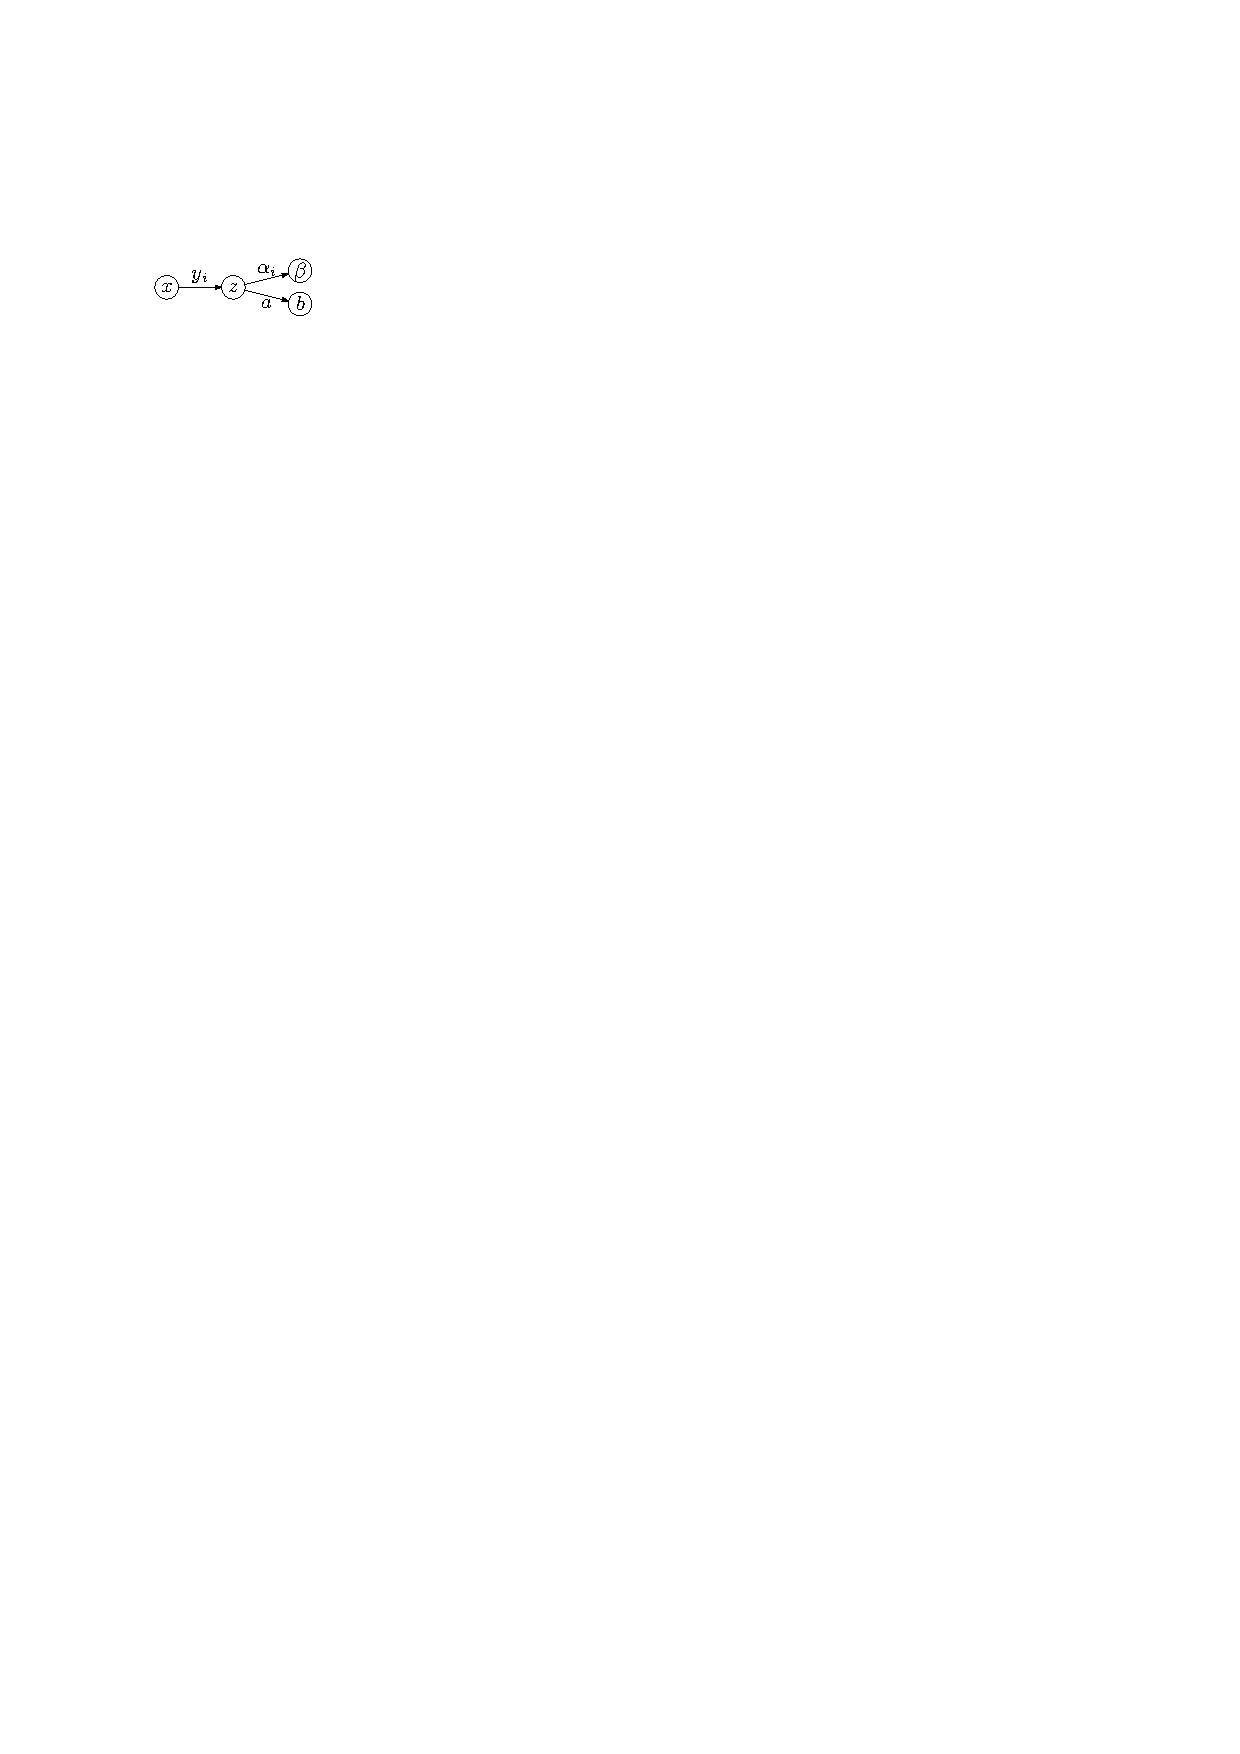
\includegraphics{push-deg3}
\end{center}

\caption{$x$ is removed from the queue. $y_i$, $z$, $a_i$, and $\alpha_i$ are never part of the queue. $\beta$ and $b$ are pushed into the queue.}
\label{fig:push-deg3}

\end{wrapfigure}


In the previous section, we described an optimized A* variant that does not push degree two nodes.
In this section, we also avoid degree three nodes.

Denote by $x,y_1,\ldots, y_k, z$ a degree chain as described in the previous section.
If $z$ is already in the queue, then $z$'s weight in the queue is adjusted as in the previous section.

If $d(z)\neq 3$ or $z$ is in the queue, our algorithm proceeds as in the previous section.
Otherwise, there exist up to two degree chains $z,a_1,\ldots,a_p,b$ and $z,\alpha_1,\ldots,\alpha_q,\beta$ such that $a_1\neq y_k \neq \alpha_1$.
Our algorithm iteratively tries to reduce all $D[a_i]$ and $D[\alpha_i]$.
If it reaches $\beta$, $\beta$'s weight in the queue is set to $D[\beta]+\pi(\beta)$.
Analogously, if $b$ is reached, $b$'s weight is set to $D[b]+\pi(b)$.
If $b$ respectively $\beta$ are not reached, our algorithm does nothing.
The situation is depicted in Figure~\ref{fig:push-deg3}.

\subsection{Avoid Dead-Ends using Largest Biconnected Component}

A lot of nodes in road networks lead to dead-ends.
Unless the source or target is is in a dead-end, it is unnecessary to explore these nodes.
This reduces the number of explored nodes and thus fewer potentials are evaluated.

In the preprocessing phase, before the CH is created, we compute the subgraph $G_C$, called \emph{core}, induced by the largested biconnected component of the undirected graph underlying $G$.
We do this using Tarjan's algorithm \cite{Tarjan's algorithm}.
For every node $v$ in the input graph $G$, we store the attachment node $a_v$ to the core.
For nodes in the core, $a_v=v$.
We exploit that all attachment nodes are single node separators and the problem can be decomposed along them.
The basic CH-potential preprocessing step is only executed for $G_C$.

The query phase is divided into four steps.
In the first step, we use Dijkstra's algorithm to explore the component that contains $s$ until $a_s$ is reached.
If this search finds $t$, then $s$ and $t$ are part of the same component.
An optimal path was found and therefore the algorithm stops early.
Otherwise, in the second step starts.
It consits of applying the basic CH-potential algorithm restricted to $G_C$ from $a_s$ to $a_t$.
Finally, in the third step, we search a path from $a_t$ towards $t$ using Dijkstra's algorithm restricted to $t$'s biconnected component.
The final path is the concatenation of all three path parts.


\section{Experiments}

\begin{itemize}
\item Avoid nothing running times, i.e., what is if $w_q = w_\ell$?
\item Multiply all weights by $\alpha$, i.e., $w_q = \alpha w_\ell$ for $\alpha$ in 1.1, 1.5, 2, 3
\item Avoid highway
\item Avoid tunnel
\item Avoid highway + tunnel
\item MapBox Live Traffic
\item Ptv-TD traffic? Achtung: Das Fass würde ich nicht aufmachen. Am Ende will ein Reviewer, dass wir avoid highway mit TD kombinieren... das ist NP-schwer
\item Running times if OSM degree 2 nodes are not extracted! Das einzige Argument pro Erhalten von Deg 2 das ich bisher kenne ist MapBox Live Traffic matchen.
\end{itemize}

Tims plan:

\begin{itemize}
\item Effectiveness of A*
	\begin{itemize}
  \item Multiplied weights by 1 to 2 in steps of 0.05
  \item On DIMACs Eur
  \item Plot x factor, y running time
  \end{itemize}

\item Algo Building Blocks
	\begin{itemize}
  \item DIMACs Eur x1.1
  \item Table
  	\begin{itemize}
    \item columns: running time, potential evals, relaxed arcs
    \item rows: (Dijkstra, SCC, Deg2, Deg3) x (CH Pot or not)
    \item or transposed?
		\end{itemize}
	\end{itemize}

\item Applications
	\begin{itemize}
  \item Table
  	\begin{itemize}
    \item columns: preprocessing time, running time, potential evals, relaxed arcs, shortest path distance / lower bound, dijkstra running time?
    \item rows: OSM Ger Mapbox Live, forbidden highways, forbidden tunnels, TD Ger06, TD Eur17, DIMACs Eur 1000 {Random|Fastest} Arcs {x2, x10}
		\end{itemize}
	\end{itemize}
\end{itemize}

\section{Conclusion}
\label{sec:conclusion}

We introduce a novel way to compute potentials for A*.
The potentials are calculated utilizing a CH on a lower bound graph and perfect with regards to that lower bound graph.
With these potentials we can speed up A* search for extended route planning problems like route planning with live traffic, time-dependent travel time predictions or user preferences.

%%
%% Bibliography
%%

%% Please use bibtex,

\bibliography{references}

% \appendix

\end{document}
